\documentclass[11pt, twoside, pdftex]{article}

% This includes all the settings that we should use for the document
\newcommand{\PDFTitle}{Simulating Verilog Designs in Quartus by Drawing Waveforms}
\newcommand{\commonPath}{../../../../Common}
\newcommand{\datePublished}{Mar 2022}

\newcommand{\versnum}{21.1} %version number quartus/AMP
\newcommand{\quartusname}{Quartus\textsuperscript{\textregistered} Prime}	
\newcommand{\textBar}{For \quartusname{} \versnum{}}
\newcommand{\thisyear}{2022 } %for copyright
\newcommand{\company}{FPGAcademy.org}
\newcommand{\longteamname}{FPGAcademy.org}
\newcommand{\teamname}{FPGAcademy}
\newcommand{\website}{FPGAcademy.org}

\newcommand{\productAcronym}{AMP}
\newcommand{\productNameShort}{Monitor Program}

\newcommand{\productNameMedTM}{Monitor Program}
\newcommand{\productNameMed}{Monitor Program}

%\newcommand{\headerLogoFilePath}[1]{#1/FPGAcademy.png}



\setlength\topmargin{-0.25in}
\setlength\headheight{0in}
\setlength\headsep{0.35in}
\setlength\textheight{8.5in}
\setlength\textwidth{7in}
\setlength\oddsidemargin{-0.25in}
\setlength\evensidemargin{-0.25in}
\setlength\parindent{0.25in}
\setlength\parskip{0in} 

\pdfpagewidth 8.5in
\pdfpageheight 11in

% listings is a package that supports encapsulating source code in LaTeX conveniently

\usepackage{listings}
% add support for graphics
\usepackage{graphicx}
\usepackage[usenames, dvipsnames]{color}

\def\expandparam\lstinputlisting[#1]#2{\edef\tmp{\noexpand\lstinputlisting[#1]{#2}}\tmp}

\widowpenalty 10000
\clubpenalty 10000

%%%%%%%%%%%%%%%%%%%% Source Code Formatting %%%%%%%%%%%%%%%%%%%%
\definecolor{globalCommentColour}{rgb}{0.588,0.588,0.588}

%%%%%%%%%%%%%%%%%%%%%%%%%%%%%%%%%%%%%%%%%%%%%%%%%%%%
% Defining a NiosII ASM highlighter for lstlisting
\lstdefinelanguage[NiosII]{Assembler} {
 	morekeywords={add, addi, and, andhi, andi, beq, bge, bgeu, bgt, bgtu, ble,  bleu, blt, bltu, bne, br, break,% 
 	bret, call, callr, cmpeq, cmpeqi, cmpge, cmpgei, cmpgeu, cmpgeui, cmpgt, cmpgti, cmpgtu, cmpgtui, cmple,%
 	cmplei, cmpleu, cmpleui, cmplt, cmplti, cmpltu, cmpltui, cmpne, cmpnei, custom, div, divu, eret, flushd,%
 	flushda, flushi, flushp, initd, initda, initi, jmp, jmpi, ldb, ldbio, ldbu, ldbuio, ldh, ldhio, ldhu, ldhuio,%
 	ldw, ldwio, mov, movhi, movi, movia, movui, mul, muli, mulxss, mulxsu, mulxuu, nextpc, nop, nor, or, orhi, ori,%
 	rdctl, rdprs, ret, rol, roli, ror, sll, slli, sra, srai, srl, srli, stb, stbio, sth, sthio, stw, stwio,%
 	sub, subi, sync, trap, wrctl, wrtcl, wrprs, xor, xori, xorhi, xori},% 	
 	morekeywords=[2]{.abort, .ABORT, .align, .app-file, .ascii, .asciz, .balign, .byte, .comm, .data, .def,%
 	.desc, .dim, .double, .eject, .else, .end, .endef, .endif, .equ, .equiv, .err, .extern, .file, .fill, .float,%
 	.global, .globl, .hword, .ident, .if, .include, .int, .irp, .irpc, .lcomm, .lflags, .line, .linkonce, .ln,%
 	.list, .long, .macro, .mri, .nolist, .octa, .org, .p2align, .psize, .quad, .rept, .sbttl, .scl, .section,%
 	.set, .short, .single, .size, .sleb128, .skip, .space, .stadb, .stabn, .stabs, .string, .symver, .tag,%
 	.text, .title, .type, .val, .uleb128, .word},% 	
 	morekeywords=[3]{et, bt, gp, sp, fp, ea, sstatus, ra, pc, status, estatus, bstatus, ienable, ipending, cpuid,%
 	exception, pteaddr, tlbacc, tlbmisc, eccinj, badaddr, config, mpubase, mpuacc},% 	
 	sensitive=t,%
 	alsoletter=.,%
	morestring=[b]",%
 	morecomment=[s]{/*}{*/},%
 	morecomment=[l]\#,%
   }[keywords,comments,strings]
   
   %% NOTE: morekeywords=[2] are GNU directives.
   
   \definecolor{niosInstructionColour}{rgb}{0.000,0.608,0.000}
   \definecolor{niosDirectiveColour}{rgb}{0.000,0.000,0.902}
   \definecolor{niosSpecialRegColour}{rgb}{0.000,0.000,0.000}
   \definecolor{niosStringColour}{rgb}{0.808,0.482,0.000}
   
   %% NOTE: To make bold use: =\bfseries\color{<colour>}
   \lstdefinestyle{defaultNiosStyle} {
   language=[NiosII]{Assembler},
   stringstyle=\color{niosStringColour},
   keywordstyle=\color{niosInstructionColour},
   keywordstyle=[2]\color{niosDirectiveColour},
   keywordstyle=[3]\itshape\color{niosSpecialRegColour}
   }
%%%%%%%%%%%%%%%%%%%%%%%%%%%%%%%%%%%%%%%%%%%%%%%%%%%%

%%%%%%%%%%%%%%%%%%%%%%%%%%%%%%%%%%%%%%%%%%%%%%%%%%%%
% Defining a ArmA9 ASM highlighter for lstlisting
\lstdefinelanguage[ArmA9]{Assembler} {
 	morekeywords={ADC, ADD, ADDS, AND, ANDS, B, BAL, BEQ, BGE, BGT, BL, BLT, BIC, BKPT, BLX, BNE, BX, CDP, CLZ, CMN, CMP, EOR,%
 	EORS, LDC, LDM, LDR, LDRB, LDRBT, LDRH, LDRSB, LDRSH, LDRT, LSL, MCR, MLA, MOV, MOVW, MOVT, MRC, MRS, MSR, MUL, MVN, ORR, PLD,%
 	ROR, RSB, RSC, SBC, SMLAL, SMULL, STC, STM, STR, STRB, STRBT, STRH, STRT, SUB, SUBS, SWI, SWP, SWPB, TEQ, UMLAL,
 	PUSH, POP, MOVS, RORS, LSR},%
 	morekeywords=[2]{.abort, .ABORT, .align, .app-file, .ascii, .asciz, .balign, .byte, .comm, .data, .def,%
 	.desc, .dim, .double, .eject, .else, .end, .endef, .endif, .equ, .equiv, .err, .extern, .file, .fill, .float,%
 	.global, .globl, .hword, .ident, .if, .include, .int, .irp, .irpc, .lcomm, .lflags, .line, .linkonce, .ln,%
 	.list, .long, .macro, .mri, .nolist, .octa, .org, .p2align, .psize, .quad, .rept, .sbttl, .scl, .section,%
 	.set, .short, .single, .size, .sleb128, .skip, .space, .stadb, .stabn, .stabs, .string, .symver, .tag,%
 	.text, .title, .type, .val, .vectors, .uleb128, .word},%
 	morekeywords=[3]{SP, PC, MIDR, CTR, TCMTR, TLBTR, MPIDR, ID_PFR0, ID_PFR1, ID_DFR0, ID_MMFR0, ID_MMFR1, ID_MMFR2,%
 	ID_MMFR3, ID_ISAR0, ID_ISAR1, ID_ISAR2, ID_ISAR3, ID_ISAR4, CCSIDR, CLIDR, AIDR, CSSELR, TTBR0, TTRB1, TTBR2, DACR,%
 	DFSR, IFSR, ADFSR, AIFSR, DFAAR, IFAR, ICIALLUIS, BPIALLIS, PAR, ICIALLU, ICIMVAU, BPIALL, DCIMVAC, DCISW, V2PCWPR,%
 	DCCVAC, DCCSW, DDIMVAC, DCISW, TLBALLIS, TLBIMVAIS, TLBIASIDIS, TLBIMVAAIS, TLBIALL, TLBIMVA, TLBIASID, TLBIMVAA,%
 	PMCR, PMCNTENSET, PMCNTENCLR, PMOVSR, PMSWINC, PMSELR, PMXEVTYPER, PMXEVCNTR, PMUSERENR, PMINTENSET, PMINTENCLR,%
 	PRRR, NRRR, PLEIDR, PLEASR, PLEFSR, PLEUAR, PLEPCR, VBAR, MVBAR, ISR, FCSEIDR, CONTEXTIDR, TPIDRURW, TPIDRURO, TPIDRPRW},%
 	sensitive=f,%
 	alsoletter=.,%
	morestring=[b]",%
 	morecomment=[s]{/*}{*/},%
 	morecomment=[l]{//},%
   }[keywords,comments,strings]
   
   %% NOTE: morekeywords=[2] are GNU directives.
   
   \definecolor{armInstructionColour}{rgb}{0.000,0.608,0.000}
   \definecolor{armDirectiveColour}{rgb}{0.000,0.000,0.902}
   \definecolor{armSpecialRegColour}{rgb}{0.000,0.000,0.000}
   \definecolor{armStringColour}{rgb}{0.808,0.482,0.000}
   
   \lstdefinestyle{defaultArmStyle} {
   language=[ArmA9]{Assembler},
   stringstyle=\color{armStringColour},
   keywordstyle=\color{armInstructionColour},
   keywordstyle=[2]\color{armDirectiveColour},
   keywordstyle=[3]\itshape\color{armSpecialRegColour}
   }
%%%%%%%%%%%%%%%%%%%%%%%%%%%%%%%%%%%%%%%%%%%%%%%%%%%%

%%%%%%%%%%%%%%%%%%%%%%%%%%%%%%%%%%%%%%%%%%%%%%%%%%%%
% Defining style for the verilog.

\definecolor{verilogCommentColour}{rgb}{0.000,0.502,0.000}

\lstdefinestyle{defaultVerilogStyle} {
language={Verilog},
keywordstyle=\color{blue},
commentstyle=\color{verilogCommentColour}
}
%%%%%%%%%%%%%%%%%%%%%%%%%%%%%%%%%%%%%%%%%%%%%%%%%%%%

%%%%%%%%%%%%%%%%%%%%%%%%%%%%%%%%%%%%%%%%%%%%%%%%%%%%
% Defining style for the vhdl.
\lstdefinestyle{defaultVHDLStyle} {
language={VHDL},
keywordstyle=\color{blue},
commentstyle=\color{verilogCommentColour}
}
%%%%%%%%%%%%%%%%%%%%%%%%%%%%%%%%%%%%%%%%%%%%%%%%%%%%

%%%%%%%%%%%%%%%%%%%%%%%%%%%%%%%%%%%%%%%%%%%%%%%%%%%%
% Java
\definecolor{javaStringColour}{rgb}{0.808,0.482,0}
%%%%%%%%%%%%%%%%%%%%%%%%%%%%%%%%%%%%%%%%%%%%%%%%%%%%

%%%%%%%%%%%%%%%%%%%%%%%%%%%%%%%%%%%%%%%%%%%%%%%%%%%%
% Defining language styles
% C
\definecolor{CStringColour}{rgb}{0.808,0.482,0}
%%%%%%%%%%%%%%%%%%%%%%%%%%%%%%%%%%%%%%%%%%%%%%%%%%%%

%%%%%%%%%%%%%%%%%%%%%%%%%%%%%%%%%%%%%%%%%%%%%%%%%%%%
% Defining extended LaTeX language.
\lstdefinelanguage[LocalLaTeX]{TeX}[LaTeX]{TeX}%
 	{moretexcs={bf, it, sf, lstset},%
   	}%

\lstdefinestyle{defaultLocalLatexStyle} {
language=[LocalLatex]{TeX},
keywordstyle=\color{blue}\bfseries,
keywordstyle=[2]\color{blue},
keywordstyle=[3]\color{blue}\bfseries
}
%%%%%%%%%%%%%%%%%%%%%%%%%%%%%%%%%%%%%%%%%%%%%%%%%%%%

\lstset{
%language = C,
%language = Verilog,
%basicstyle=\color{black}\rmfamily\ttfamily,
basicstyle=\small\color{black}\ttfamily,
commentstyle=\small\color{globalCommentColour}\itshape\ttfamily,
keywordstyle=\small\color{blue}\bfseries\ttfamily,
showstringspaces=false,
frame=none, %lines % boxed listings
breaklines=true,
breakatwhitespace=true,
tabsize=4
}
%%%%%%%%%%%%%%%%%%%%%%%%%%%%%%%%%%%%%%%%%%%%%%%%%%%%%%%%%%%%%%%%


%\usepackage[centering]{geometry}.
%%%%%%%%%%%%%%%%%%%%%%%%%%%%%%%%%%%%%%%%%%%%%%%%%%%
% Document Settings
\usepackage[labelsep=period]{caption}
% we can choose a better font later
%\usepackage{palatino}
\usepackage{fourier}
%\fontencoding{T1}
% include common used symbols
\usepackage{textcomp}
% add support for graphics
\usepackage{graphicx}
\usepackage[usenames, dvipsnames]{color}
% enable to draw thick or thin table hlines
\setlength{\doublerulesep}{\arrayrulewidth}
\usepackage{longtable}
\setlongtables
%\usepackage{array}
% It may be better to use PDFLaTeX as it can generate bookmarks for the
% document

% Add some useful packages
\usepackage{ae,aecompl}
\usepackage{epsfig,float,times}

% reset the font for section
\usepackage{sectsty}
%\allsectionsfont{\fontfamily{ptm}\selectfont}
\allsectionsfont{\usefont{OT1}{phv}{bc}{n}\selectfont}

% use compact space for sections
\usepackage[compact]{titlesec}
\titlespacing{\section}{0pt}{0.2in}{*0}
\titlespacing{\subsection}{0pt}{0.1in}{*0}
\titlespacing{\subsubsection}{0pt}{0.05in}{*0}

% fancyhdr header and footer customization
\usepackage{layout}
\usepackage{fancyhdr}
\pagestyle{fancy}
\fancyhead{}
\fancyhead[R]{\textit{\tiny{\textBar}}}
\fancyfoot{}
\fancyfoot[LO,
RE]{\textrm{\href{https://www.fpgacademy.org}{\small \longteamname}} \\ {\small \datePublished }}
\fancyfoot[RO, LE]{\small \thepage}
% two-side settings
%\fancyhead{} % clear all header fields
%\fancyfoot{} % clear all footer fields
%\fancyfoot[LE,RO]{\thepage}
\renewcommand{\headrulewidth}{2pt}
\renewcommand{\headrule}{{\color{blue} \hrule width\headwidth height\headrulewidth \vskip-\headrulewidth}}
\renewcommand{\footrulewidth}{0pt}

% Format the footer on page 1
\fancypagestyle{plain}{
\fancyhead{}
\fancyfoot{}
\fancyfoot[LO,
RE]{\textrm{\href{https://www.fpgacademy.org}{\small \longteamname}} \\ {\small \datePublished }}
\fancyfoot[RO, LE]{\small \thepage}
\renewcommand{\headrulewidth}{0pt}
}
% adjust some setting to try to make the figure stay in the same page with text
% Reference: 	http://www.cs.uu.nl/~piet/floats/node1.html
%   			http://mintaka.sdsu.edu/GF/bibliog/latex/floats.html
%   General parameters, for ALL pages:
\renewcommand{\topfraction}{0.9}	% max fraction of floats at top
\renewcommand{\bottomfraction}{0.8}	% max fraction of floats at bottom
%   Parameters for TEXT pages (not float pages):
\setcounter{topnumber}{3}
\setcounter{bottomnumber}{3}
\setcounter{totalnumber}{5}     % 2 may work better
\setcounter{dbltopnumber}{2}    % for 2-column pages
\renewcommand{\dbltopfraction}{0.9}	% fit big float above 2-col. text
\renewcommand{\textfraction}{0.07}	% allow minimal text w. figs
%   Parameters for FLOAT pages (not text pages):
\renewcommand{\floatpagefraction}{0.7}	% require fuller float pages
% N.B.: floatpagefraction MUST be less than topfraction !!
\renewcommand{\dblfloatpagefraction}{0.7}	% require fuller float pages
%%%%%%%%%%%%%%%%%%%%%%%%%%%%%%%%%%%%%%%%%%%%%%%%%%%
% remember to use [htp] or [htpb] for placement
%%%%%%%%%%%%%%%%%%%%%%%%%%%%%%%%%%%%%%%%%%%%%%%%%%%

% set no indent for paragraph
\setlength{\parindent}{0em}
\addtolength{\parskip}{11pt}
\newcommand{\compact}{[topsep=0pt]}
% use this package to reduce space
\usepackage{enumitem}
\usepackage{multirow}
\usepackage{rotating}
\usepackage{pifont}
\usepackage{dingbat}
\newcommand{\itemsecond}{$\circ$}
%
%%%%%%%%%%%%%%%%%%
\date{}
\author{}
%%%%%%%%%%%%%%%%%%
\newcommand{\de}{DE-series}
\newcommand{\up}{FPGAcademy}
\newcommand{\fabric}{Avalon Switch Fabric}
\newcommand{\TODO}[1]{\textcolor{red}{\textbf{TODO}: #1}}
\def\registered{{\ooalign{\hfil\raise .00ex\hbox{\scriptsize R}\hfil\crcr\mathhexbox20D}}}

% enable url and reference(bookmarks) in pdf
\usepackage{url}
\usepackage[pdftex, colorlinks]{hyperref}
\hypersetup{%
pdftitle={\PDFTitle},
linkcolor=blue,
hyperindex=true,
pdfauthor={\longteamname},
pdfkeywords={FPGAcademy, Academic Program, Example System},
bookmarksnumbered,
bookmarksopen=false,
filecolor=blue,
pdfstartview={FitH},
urlcolor=blue,
plainpages=false,
pdfpagelabels=true,
linkbordercolor={1 1 1} %no color for link border
}%
%%%%%%%%%%%%%%%%%%%%%%%%%%%%%%%%%%%%%%%%%%%%%%%%%%%
\setlength{\fboxsep}{0.7pt}
\setlength{\fboxrule}{0.5pt}

\newcommand{\red}[1]{{\color{red}\sf{#1}}}
\newcommand{\blue}[1]{{\color{blue}\sf{#1}}}



\usepackage{placeins}

%%%%%%%%%%%%%%%%%%%%%%%%%
% Add title
\newcommand{\doctitle}{Simulating Verilog Designs in \\ Quartus by Drawing Waveforms}
\newcommand{\dochead}{Simulating Verilog Designs in Quartus by Drawing Waveforms}
% Usually no need to change these two lines
\title{\fontfamily{phv}\selectfont{\doctitle} }
\chead{ \small{\textsc{\bfseries \dochead} } }
% Customizations
%%%%%%%%%%%%%%%%%%%%%%%%%
% Allows multiple figures per page

\renewcommand\floatpagefraction{.9}
\renewcommand\topfraction{.9}
\renewcommand\bottomfraction{.9}
\renewcommand\textfraction{.1}   
\setcounter{totalnumber}{50}
\setcounter{topnumber}{50}
\setcounter{bottomnumber}{50}
\widowpenalty 10000
\clubpenalty 10000
\raggedbottom

%%%%%%%%%%%%%%%%%%
%%% DOCUMENT START
%\begin{document}
\begin{document}
\begin{table}
    \centering
    \begin{tabular}{p{5cm}p{4cm}}
	\hspace{-3cm}
        &
        \raisebox{1\height}{\parbox[h]{0.5\textwidth}{\Large\fontfamily{phv}\selectfont{\textsf{\doctitle}}}}
    \end{tabular}
    \label{tab:logo}
\end{table}

\colorbox[rgb]{0,0.384,0.816}{\parbox[h]{\textwidth}{\color{white}\textsf{\textit{\textBar}}}}

\thispagestyle{plain}
\newcommand{\red}[1]{{\color{red}\sf{#1}}}
\lstset{language = Verilog}
 
\section{Introduction}

An effective way of determining the correctness of a logic circuit is to simulate its behavior.
This tutorial provides an introduction to such simulation using the 
Altera\textsuperscript{\textregistered} Quartus\textsuperscript{\textregistered} Prime system.

The simulation method used in this tutorial is based on drawing waveforms, similar to
timing diagrams. These waveforms are drawn using a Waveform Editor tool in the Quartus
system. The system then automatically converts the waveforms into a simulation {\it
testbench}, which is simulated by executing the {\it ModelSim-Altera} application
software. The outputs from ModelSim are then converted back into waveforms that are displayed 
by the Quartus Waveform Editor tool.  This tutorial is intended for beginner students.
We show how to use the Waveform Editor tool to perform a simulation of a circuit specified in 
the Verilog hardware description language.  Only a very basic understanding of Verilog is 
needed for this purpose. 

{\bf Contents}:
\begin{itemize}
\item Design Project
\item Creating Waveforms for Simulation
\item Simulation
\item Making Changes and Resimulating
\item Concluding Remarks
\end{itemize}
\clearpage
\newpage

The Waveform Editor tool included with the Quartus prime software allows the user to apply 
inputs to the designed circuit, usually referred to as {\it test vectors}, in the form of 
waveforms and to observe the outputs generated in response. 
~\\

In this tutorial, the reader will learn about:
\begin{itemize}
\item Test vectors needed to test the designed circuit
\item Using the Waveform Editor tool to draw test vector waveforms
\item Functional simulation, which is used to verify the functional 
correctness of a synthesized circuit
\item Timing simulation, which is used to verify the timing of signals in a synthesized circuit
\end{itemize}

This tutorial is aimed at the reader who wishes to simulate circuits defined
by using the Verilog hardware description language. An equivalent tutorial is
available for the user who prefers the VHDL language.

\section{Design Project}
\label{sec:design_project}
To illustrate the simulation process, we will use a very simple logic circuit that 
implements the {\it majority} function of three inputs, $x_1$, $x_2$ and $x_3$. The circuit
is defined by the expression
$$
f(x_1, x_2, x_3) = x_1 x_2 + x_1 x_3 + x_2 x_3
$$
\noindent
In Verilog, this circuit can be specified as follows:

\lstset{language=Verilog} 
\begin{center}
\begin{lstlisting}
module majority3 (x1, x2, x3, f);
	input	x1, x2, x3;
	output	f;
	assign	f = (x1 & x2) | (x1 & x3) | (x2 & x3);
endmodule 
\end{lstlisting}
\end{center}


\noindent
~\\
Implement this circuit as follows:
\begin{itemize}
\item Create a new Quartus Prime project, named {\it majority3}.
\item Include a file {\it majority3.v}, which provides the Verilog code shown above.
\item Optionally, select a desired FPGA device when making your Quartus project. This step 
is important only if you are intending to implement the designed circuit in an FPGA board. 
A list of device names for several boards can be found in Table~\ref{tab:device}.
\item Compile your project.
\end{itemize}

\begin{table}[H]
	\begin{center}
	\begin{tabular}{| c | c |}
	\hline
	Board & Device Name \\
	\hline
	DE0-CV & Cyclone\textsuperscript{\textregistered} V 5CEBA4F23C7 \\
	\hline
	DE0-Nano & Cyclone\textsuperscript{\textregistered} IVE EP4CE22F17C6 \\
	\hline
	DE0-Nano-SoC & Cyclone\textsuperscript{\textregistered} V SoC 5CSEMA4U23C6 \\
	\hline
	DE1-SoC & Cyclone\textsuperscript{\textregistered} V SoC 5CSEMA5F31C6 \\
	\hline
	DE2-115 & Cyclone\textsuperscript{\textregistered} IVE EP4CE115F29C7 \\
	\hline
	DE10-Lite & Max\textsuperscript{\textregistered} 10 10M50DAF484C7G \\
	\hline
	DE10-Standard & Cyclone\textsuperscript{\textregistered} V SoC 5CSXFC6D6F31C6 \\
	\hline
	DE10-Nano & Cyclone\textsuperscript{\textregistered} V SE 5CSEBA6U2317 \\
	\hline
	\end{tabular}
	\caption{DE-series FPGA device names}
	\label{tab:device}
	\end{center}
\end{table}

\section{Creating Waveforms for Simulation}
\label{sec:creating_waveforms_for_simulation}

To create test vectors for your design, select {\sf File $>$ New... $>$ Verification/Debugging Files $>$ University Program VWF} in the Quartus Prime window where the design project is open.
This opens the Simulation Waveform Editor tool, shown in Figure~\ref{fig:5}, which allows you to specify the desired input waveforms.

\begin{figure}[H]
   \begin{center}
      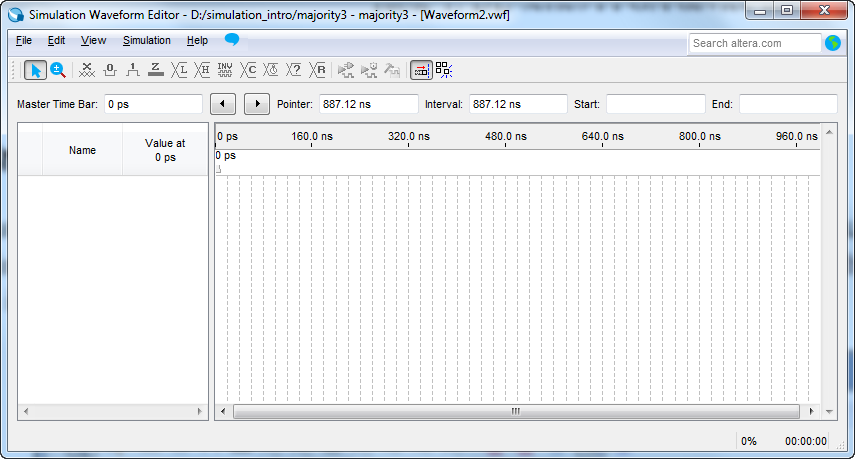
\includegraphics[scale=0.65]{figures/figure5.png}
   \caption{The Waveform Editor window.} 
	 \label{fig:5}
	 \end{center}
\end{figure}

For our simple circuit, we can do a complete simulation by applying all eight possible valuations of the 
input signals $x_1$, $x_2$ and $x_3$. 
The output {\it f} should then display the logic values defined by
the truth table for the majority function.

We will run the simulation for 800 ns; so, select {\sf Edit $>$ Set End Time...} in the
Waveform Editor and in the
pop-up window that will appear specify the time of 800 ns, and click {\sf OK}. 
This will adjust the time scale in the window of Figure~\ref{fig:5}.  

Before drawing the input waveforms, it is necessary to locate the desired signals in the
implemented circuit. In FPGA jargon, the term ``node'' is used to refer to a signal in 
a circuit. This could be an input signal (input node), output signal (output node), or
an internal signal. For our task, we need to find the input and output nodes. This is done
by using a utility program called the Node Finder.

In the Waveform Editor window, select {\sf Edit $>$ Insert $>$ Insert Node or Bus...}. In the
pop-up window that appears, which is shown in Figure~\ref{fig:6}, click on {\sf Node Finder}.
~\\

\begin{figure}[H]
   \begin{center}
      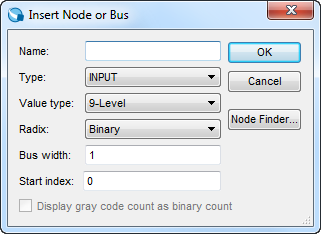
\includegraphics[scale=0.7]{figures/figure6.png}
   \caption{The Insert Node or Bus dialog.} 
	 \label{fig:6}
	 \end{center}
\end{figure}

The Node Finder window is presented in Figure~\ref{fig:7}. A filter is used to identify the nodes of interest.
In our circuit, we are only interested in the nodes that appear on the {\it pins} (i.e. external
connections) of the FPGA chip. Hence, the filter setting should be {\sf Pins: all}. Click on
{\sf List}, which will display the nodes as indicated in the figure. In a large circuit there could 
be many nodes displayed. We need to select the nodes that we wish to observe in the simulation.
This is done by highlighting the desired nodes and clicking on the {\sf >} button. Select the nodes
labeled {\it x1}, {\it x2}, {\it x3}, and {\it f}, which will lead to the image in Figure~\ref{fig:8}.
Click {\sf OK} in this window and also upon return to the window in Figure~\ref{fig:6}. This returns to
the Waveform Editor window, with the selected signals included as presented in Figure~\ref{fig:9}.

\begin{figure}[H]
   \begin{center}
      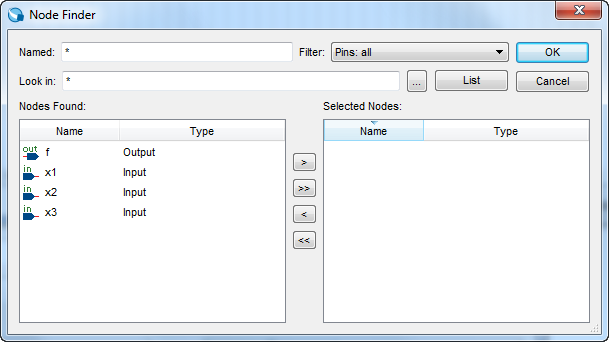
\includegraphics[scale=0.65]{figures/figure7.png}
   \caption{The Node Finder dialog.} 
	 \label{fig:7}
	 \end{center}
\end{figure}

\begin{figure}[H]
   \begin{center}
      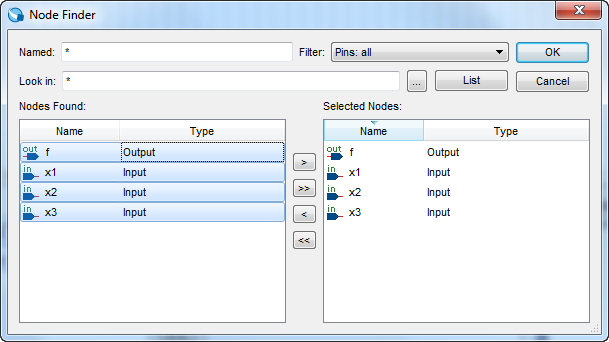
\includegraphics[scale=0.65]{figures/figure8.png}
   \caption{The selected signals.} 
	 \label{fig:8}
	 \end{center}
\end{figure}

Observe that in Figure~\ref{fig:9} all input signals are at logic level 0. The output, {\it f}
is shown as undefined. Next, we have to draw the input waveforms. Then, we will simulate
the circuit, which will produce the output waveform.

To make it easier to draw the input waveforms, the Waveform Editor displays dashed grid lines.
The spacing of the grid lines can be adjusted by selecting {\sf Edit $>$ Grid Size...}, and in the
pop-up box in Figure~\ref{fig:10} specifying the desired size. The spacing of grid lines in Figure~\ref{fig:9} is
20 ns. Another convenience in drawing is to have transitions of a waveform snap on 
grid lines. This feature is activated by clicking on the {\sf Snap to Grid} icon 
\hbox{
\includegraphics[scale=0.7]{figures/icon1.png}}, or by selecting the command
{\sf Edit $>$ Snap to Grid}.
~\\

\begin{figure}[H]
   \begin{center}
      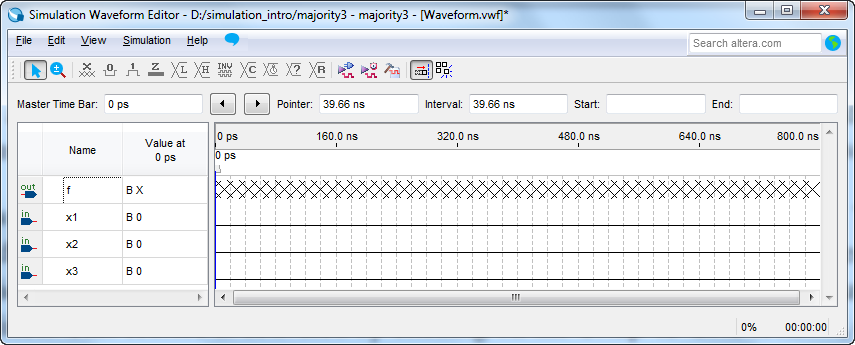
\includegraphics[scale=0.65]{figures/figure9.png}
   \caption{Signals in the Waveform Editor window.} 
	 \label{fig:9}
	 \end{center}
\end{figure}

\begin{figure}[H]
   \begin{center}
      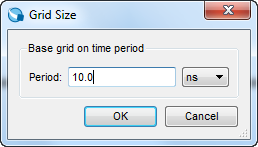
\includegraphics[scale=0.7]{figures/figure10.png}
   \caption{Specifying the grid spacing.} 
	 \label{fig:10}
	 \end{center}
\end{figure}

Input waveforms can be drawn in different ways. The most straightforward way is to indicate a
specific time range and specify the value of a signal. To illustrate this approach, click the
mouse on the {\it x1} waveform near the 400-ns point and then drag the mouse to the 800-ns point. 
The selected time interval will be highlighted in blue, as depicted in Figure~\ref{fig:11}. 
Change the value of the waveform to 1 by
clicking on the {\sf Forcing High (1)} icon \hbox{
\includegraphics[scale=0.7]{figures/icon2.png}}, as illustrated 
in Figure~\ref{fig:12}.
~\\

\begin{figure}[H]
   \begin{center}
      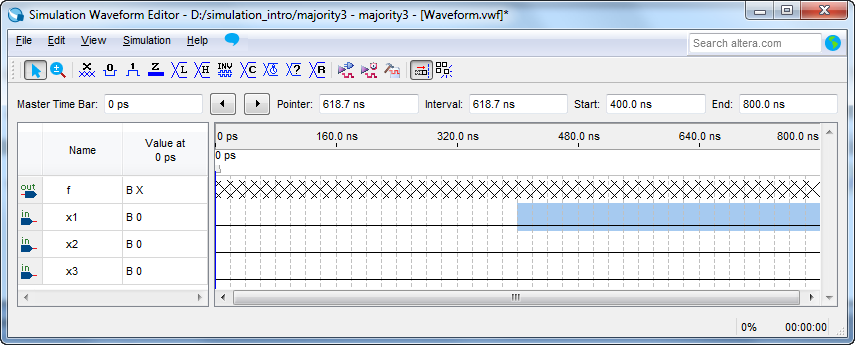
\includegraphics[scale=0.65]{figures/figure11.png}
   \caption{Selection of a time interval.} 
	 \label{fig:11}
	 \end{center}
\end{figure}

\begin{figure}[H]
   \begin{center}
      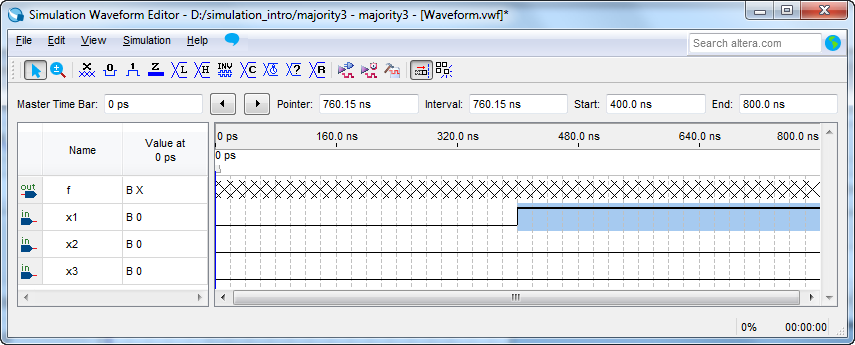
\includegraphics[scale=0.65]{figures/figure12.png}
   \caption{Drawing the waveform for {\it x1}} 
	 \label{fig:12}
	 \end{center}
\end{figure}

In creating the waveform for {\it x1}, we used the icon \hbox{
\includegraphics[scale=0.7]{figures/icon2.png}}
to implement the logic value 1. Another possibility is to invert the value of the signal
in a selected time interval by using the {\sf Invert} icon \hbox{
\includegraphics[scale=0.7]{figures/icon3.png}}.
We will use this approach to create the waveform for {\it x2}, which should change from 
0 to 1 at 200 ns, then back to 0 at 400 ns, and again to 1 at 600 ns.  
Select the interval from 200 to 400 ns and click on the icon. 
Then do the same for the interval from 600 to 800 ns, as illustrated in Figure~\ref{fig:13}.
~\\

\begin{figure}[H]
   \begin{center}
      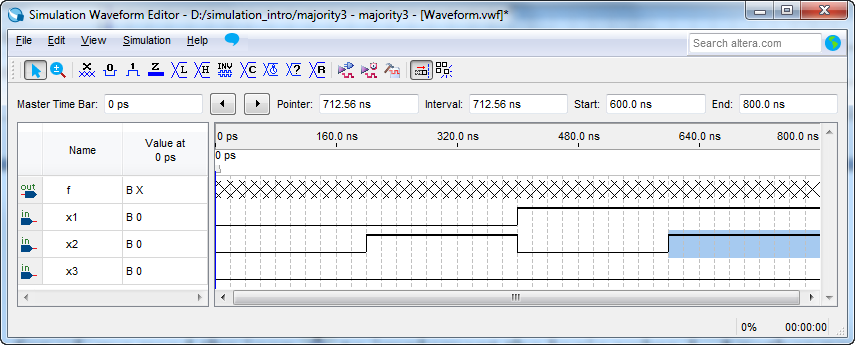
\includegraphics[scale=0.65]{figures/figure13.png}
   \caption{Drawing the waveform for {\it x2}.} 
	 \label{fig:13}
	 \end{center}
\end{figure}

We will use a third approach to draw the waveform for {\it x3}. This signal
should alternate between logic values 0 and 1 at each 100-ns interval.
Such a regular pattern is indicative of a {\it clock} signal that is used in many logic circuits.
Even though there is no clock signal in our example circuit, 
it is convenient to specify {\it x3} in this manner.
Click on the {\it x3} input, which selects the entire 800-ns interval. Then, click on the
{\sf Overwrite Clock} icon \hbox{
\includegraphics[scale=0.7]{figures/icon4.png}}, as 
indicated in Figure~\ref{fig:14}.  This leads to the pop-up window in Figure~\ref{fig:15}. 
Specify the clock period of 200 ns and the duty
cycle of 50\%, and click {\sf OK}. The result is depicted in Figure~\ref{fig:16}.
~\\

\begin{figure}[H]
   \begin{center}
      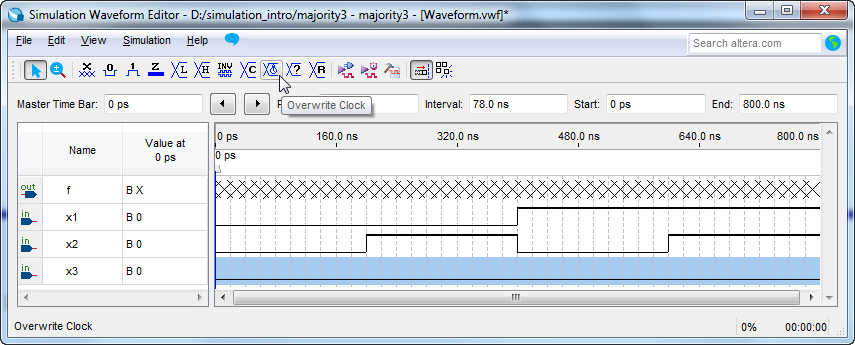
\includegraphics[scale=0.65]{figures/figure14.png}
   \caption{Drawing the waveform for {\it x3}.} 
	 \label{fig:14}
	 \end{center}
\end{figure}

\begin{figure}[H]
   \begin{center}
      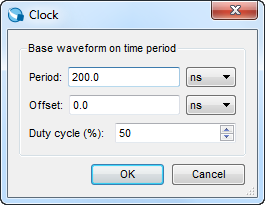
\includegraphics[scale=0.7]{figures/figure15.png}
   \caption{Defining the clock characteristics} 
	 \label{fig:15}
	 \end{center}
\end{figure}

\begin{figure}[H]
   \begin{center}
      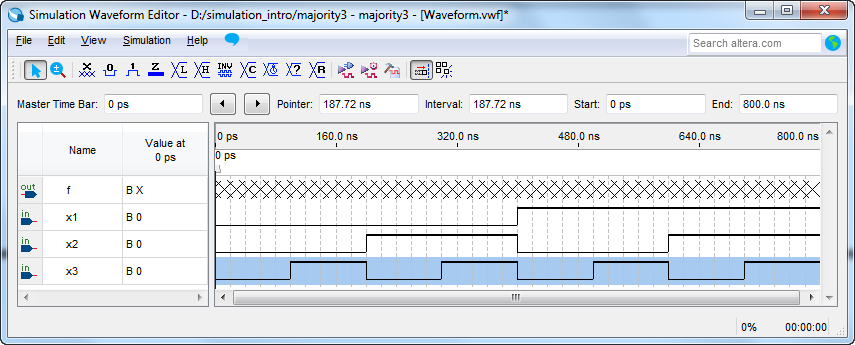
\includegraphics[scale=0.65]{figures/figure16.png}
   \caption{The completed input waveforms.} 
	 \label{fig:16}
	 \end{center}
\end{figure}

Save the waveform file as {\it Waveform.vwf}.
Note that the suffix {\it vwf} stands for {\it vector waveform file}. VWF files that are 
added to the Quartus Prime project can be accessed at any time in the
Project Navigator Widget's Files tab.

\section{Simulation}

The Simulation Waveform Editor performs the simulation by using the simulation tool known as
{\it ModelSim}.  ModelSim-Intel Edition is strongly recommended for use with the Simulation 
Waveform Editor, as it contains the Intel device libraries necessary for simulations. To 
use a standard version of ModelSim, the path to its executables must be specified in the
Quartus Prime software under {\sf Tools $>$ Options... $>$ EDA Tool Options}. If both ModelSim and 
ModelSim-Intel are available, the simulator will preferentially use ModelSim-Intel.

\subsection{Functional Simulation}

Now that we have created the input vector waveform, we can simulate the circuit. 
In the Simulation Waveform Editor, select {\sf Simulation $>$ Run Functional Simulation},
or click on the icon \hbox{
\includegraphics[scale=0.8]{figures/icon6.png}}. A pop-up window 
will show the progress of the simulation, then automatically close when it is complete. A 
second Simulation Waveform Editor window then opens the output waveform, as depicted in 
Figure~\ref{fig:17}. The output waveform is read-only, so any changes in simulation have 
to be done by modifying the {\it Waveform.vwf} file and resimulating the circuit.
Observe that the output {\it f} is equal to 1 whenever two or three inputs have 
the value 1, which verifies the correctness of our design.
~\\

\begin{figure}[H]
   \begin{center}
      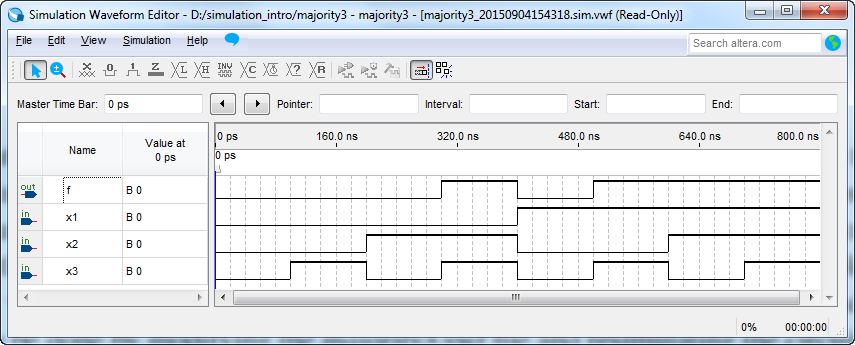
\includegraphics[scale=0.65]{figures/figure17.png}
   \caption{Result of the functional simulation.} 
	 \label{fig:17}
	 \end{center}
\end{figure}

\subsection{Timing Simulation}

To observe the actual propagation delays in our circuit, we have to perform a timing simulation.
(Note that for FPGA devices with preliminary timing models that the timing simulation results
may be the same as functional simulation results.)
In the Simulation Waveform Editor, select {\sf Simulation $>$ Run Timing Simulation},
or click on the icon \hbox{
\includegraphics[scale=0.9]{figures/icon7.png}}. A pop-up window 
will show the progress of the simulation, then automatically close when it is complete. A 
second Simulation Waveform Editor window then opens the output waveform. The output waveform 
is read-only, so any changes in simulation have to be done by modifying the {\it Waveform.vwf}
file and resimulating the circuit.
~\\

The timing simulation shows that there are delays when signals change from one value to another. 
Figure~\ref{fig:21} shows the waveform, zoomed in at 300 ns to show the propagation delay 
between {\it x3} and {\it f}. The waveform indicates that the maximum delay is approximately 6 ns. 
~\\

{\bf Note:} timing simulations are only supported by Cyclone IV\textsuperscript{\textregistered} and Stratix IV\textsuperscript{\textregistered} FPGAs.
If your Quartus project is not setup for a Cyclone IV or Stratix IV device, the result of running a timing simulation will be identical to the functional simulation.

\begin{figure}[H]
   \begin{center}
      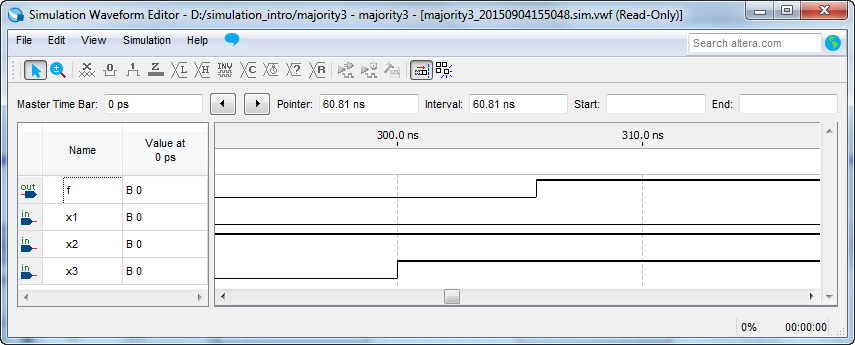
\includegraphics[scale=0.65]{figures/figure21.png}
   \caption{Result of the timing simulation, zoomed in at 300 ns.} 
	 \label{fig:21}
	 \end{center}
\end{figure}

\section{Making Changes and Resimulating}

Changes in the input waveforms can be made using the approaches explained above. The circuit
can then be resimulated using the altered waveforms. For example, change the
waveform for $x_1$ to have the logic value 1 in the interval from 100 to 240 ns, as indicated
in Figure~\ref{fig:18}. Now, simulate the circuit again. The result is 
given in Figure~\ref{fig:19}. If errors in the circuit are discovered, then these errors can be fixed by
changing the Verilog code and recompiling the design using the Quartus Prime software.
~\\

\begin{figure}[H]
   \begin{center}
      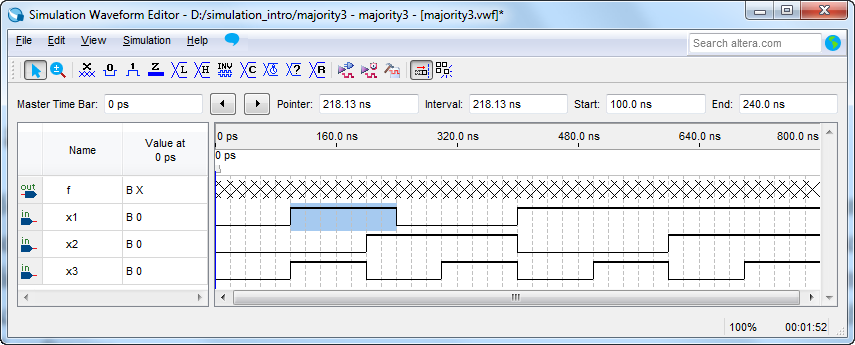
\includegraphics[scale=0.65]{figures/figure18.png}
   \caption{Modified input waveforms.} 
	 \label{fig:18}
	 \end{center}
\end{figure}

\begin{figure}[H]
   \begin{center}
      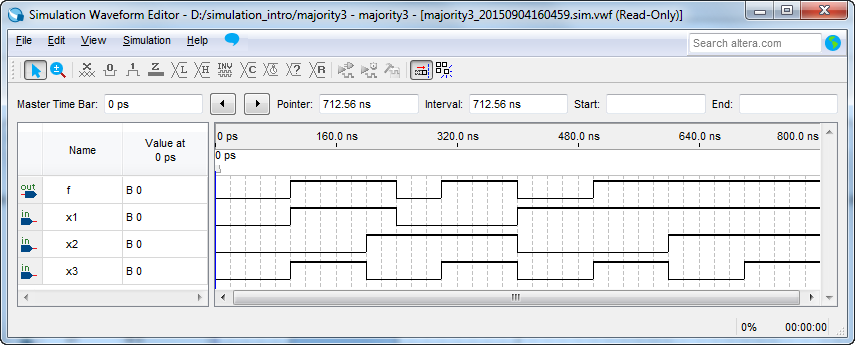
\includegraphics[scale=0.65]{figures/figure19.png}
   \caption{Result of the new simulation.} 
	 \label{fig:19}
	 \end{center}
\end{figure}


\section{Concluding Remarks}

The purpose of this tutorial is to provide a quick introduction to the Simulation Waveform Editor, 
explaining only the rudimentary aspects of functional and timing simulations. Details about 
additional features of the Simulation Waveform Editor can be found in the appendix of this document. 
The reader may also want to learn how to directly simulate circuits using ModelSim, rather
than simulating via the Quartus Prime software as done in this tutorial. It is possible to
draw waveforms using a ModelSim waveform editing tool, as described in the tutorial
{\it Using ModelSim by Drawing Waveforms}.  It is also possible to provide ModelSim inputs
by writing a Verilog testbench, as described in the tutorial
{\it Using ModelSim with Testbenches}. These tutorials are available in the
\texttt{Digital Logic Simulation and Debug} section of the \texttt{Tutorials} tab on the 
{\href{https://www.fpgacademy.org/tutorials.html} {FPGAcademy.org}} website.

\newpage
\appendix
\setcounter{figure}{0}
\setcounter{table}{0}

\section{Simulation Waveform Editor}
In section \ref{sec:creating_waveforms_for_simulation} we introduced the Waveform Editor tool, which is used to view and edit waveforms 
that are used in simulation. Additional features of the Waveform Editor are described in this appendix.

\subsection{Waveform Editor Toolbar}
The Waveform Editor window is illustrated in Figure~\ref{fig:fig1}. The tool includes several commands 
which can be accessed by using the mouse, including {\sf File}, {\sf Edit}, {\sf View}, {\sf Simulation}, and {\sf Help}. 
Below these commands, as shown in the figure, there is a toolbar that contains a number of icons which are useful when manipulating waveforms. 
This toolbar should be visible by default, but if it is not visible, then right-click near the top of the window 
(below the title bar) and select {\sf Waveform Editor} in the menu that appears.

The toolbar icons are described below.

\begin{description}
	\item {\sf Selection Tool} \hbox{
\includegraphics[scale=0.7]{figures/appendix/icon1.png}}\\
	This tool is used to select waveform intervals and apply changes. To make a 
	selection, click on any part of a waveform and drag the blue box across the 
	desired interval. It's possible to select multiple waveforms at the same time, as shown in Figure~\ref{fig:fig1},
	or select entire waveform(s) by clicking on its name(s).\\
	\begin{figure}[H]
	   \begin{center}
	      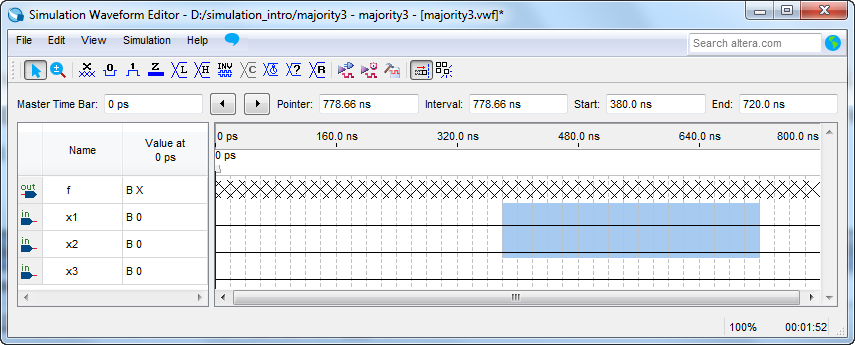
\includegraphics[scale=0.65]{figures/appendix/figure1.png}
	   \caption{Using the Selection Tool to select a portion of multiple waveforms.} 
		 \label{fig:fig1}
		 \end{center}
	\end{figure}
	
	Double clicking the selection tool anywhere on a waveform will 
	select the largest interval with the same value from where the cursor points. Double clicking on  
	a selected interval brings up the window to set arbitrary values for that interval. 

	\item {\sf Zoom Tool} \hbox{
\includegraphics[scale=0.7]{figures/appendix/icon2.png}}\\
	This tool is used to zoom in or zoom out in the waveform display, as indicated in Figure~\ref{fig:fig2}. 
	Left-clicking zooms into the display and right-clicking zooms out.
	\begin{figure}[H]
	   \begin{center}
	      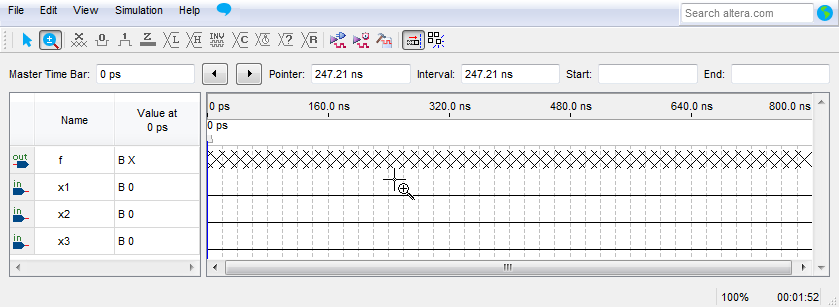
\includegraphics[scale=0.65]{figures/appendix/figure2.png}
	   \caption{Using the Zoom Tool.} 
		 \label{fig:fig2}
		 \end{center}
	\end{figure}
	
	\item {\sf Forcing Unknown(X)} \hbox{
\includegraphics[scale=0.7]{figures/appendix/icon3.png}}\\
	This tool allows the selected part of a waveform to be set to the value {\sf Unknown (x)}. An example is given
	in Figure~\ref{fig:fig3}, using the majority3 function circuit that was described in section \ref{sec:design_project}. 
	The value of the signal {\it x3} has been set to unknown for the first half of the simulation. 
	Running the simulation with these input values results in the output waveform {\it f} that is shown in the figure. 
	Note that the value of {\it f} is unknown between 200 to 400 ns. 
	\begin{figure}[H]
	   \begin{center}
	      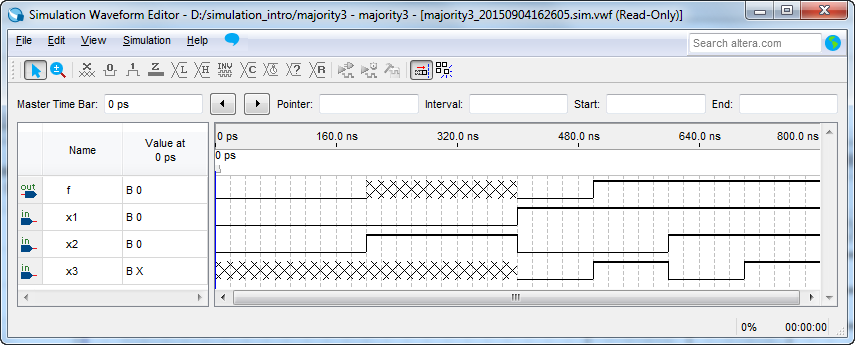
\includegraphics[scale=0.65]{figures/appendix/figure3.png}
	   \caption{Setting the value of an input to {\sf Unknown (X)}.} 
		 \label{fig:fig3}
		 \end{center}
	\end{figure}	

	\item {\sf Forcing Low (0)} \hbox{
\includegraphics[scale=0.7]{figures/appendix/icon4.png}} {\sf and Forcing High(1)} \hbox{
\includegraphics[scale=0.7]{figures/appendix/icon5.png}}\\
	These tools are used to force the selected part of a waveform to the value low (0) or high (1), as shown in Figures~\ref{fig:fig4} 
	and \ref{fig:fig5}, respectively. 
	\begin{figure}[H]
	   \begin{center}
	      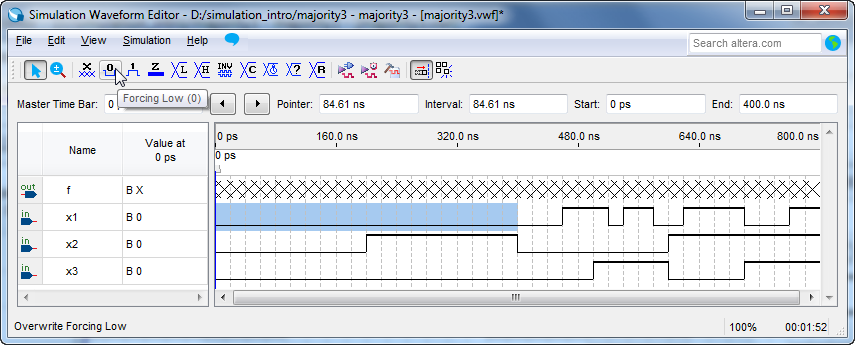
\includegraphics[scale=0.65]{figures/appendix/figure4.png}
	   \caption{Forcing $x_1$ to be low from 0 to 400 ns.} 
		 \label{fig:fig4}
		 \end{center}
	\end{figure}	
	
	\begin{figure}[H]
	   \begin{center}
	      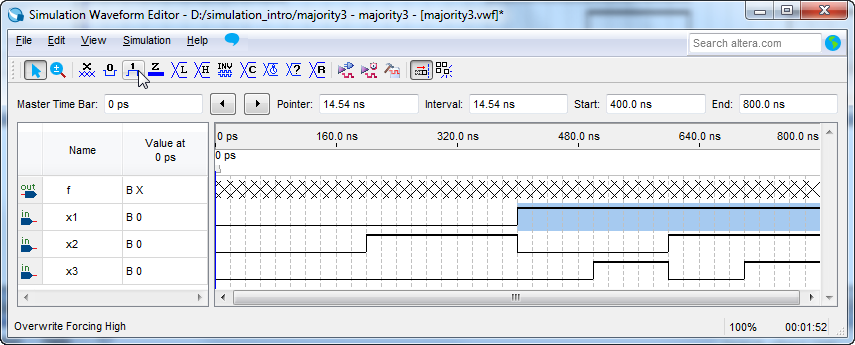
\includegraphics[scale=0.65]{figures/appendix/figure5.png}
	   \caption{Forcing $x_1$ to be high from 400 to 800 ns.} 
		 \label{fig:fig5}
		 \end{center}
	\end{figure}	
	
	\item {\sf High Impedance (Z)} \hbox{
\includegraphics[scale=0.7]{figures/appendix/icon6.png}}\\
	This tool forces the selected waveform to the value {\sf High Impedance (Z)}, as shown in Figure~\ref{fig:fig6}. 
	The high impedance value represents a signal that has not been set to any specific value---that is, an input pin 
	that is not connected. Forcing output waveforms to have high impedance does not affect the 
	output simulation waveforms.
	\begin{figure}[H]
	   \begin{center}
	      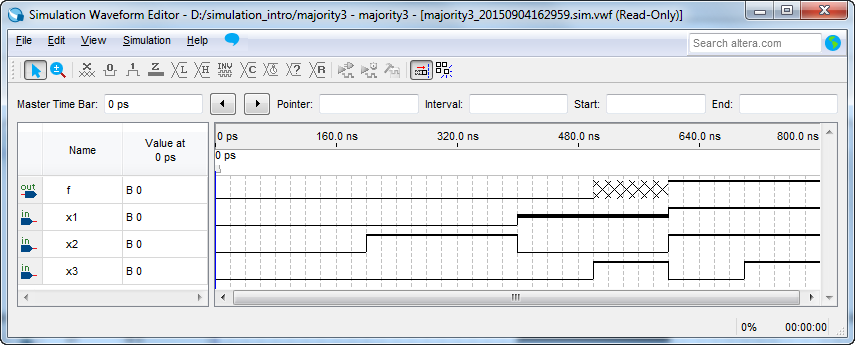
\includegraphics[scale=0.65]{figures/appendix/figure6.png}
	   \caption{Setting a signal to high impedance.} 
		 \label{fig:fig6}
		 \end{center}
	\end{figure}
	
	\item {\sf Weak Low (L)} \hbox{
\includegraphics[scale=0.7]{figures/appendix/icon7.png}} {\sf and Weak High (H)} \hbox{
\includegraphics[scale=0.7]{figures/appendix/icon8.png}}\\
	These tools are used to set a signal to the values {\sf Weak Low (L)} or {\sf Weak High (H)}, which represents 
	a circuit in which a bidirectional signal is pulled down or up by using a resistor. Examples are shown in 
	Figures \ref{fig:fig7} and \ref{fig:fig8}.
	\begin{figure}[H]
	   \begin{center}
	      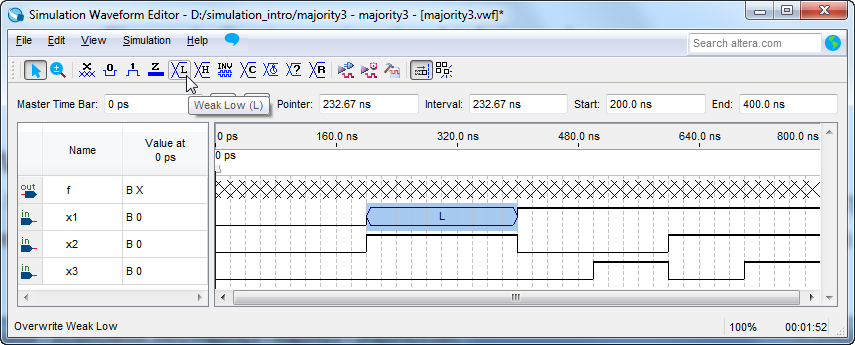
\includegraphics[scale=0.65]{figures/appendix/figure7.png}
	   \caption{Changing the {\it x1} signal to be weak low from 200 to 400 ns.} 
		 \label{fig:fig7}
		 \end{center}
	\end{figure}		
	\begin{figure}[H]
	   \begin{center}
	      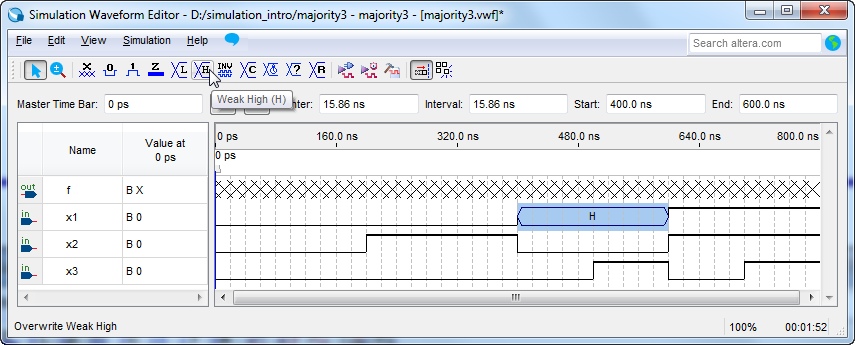
\includegraphics[scale=0.65]{figures/appendix/figure8.png}
	   \caption{Changing the {\it x1} signal to be weak high from 400 to 600 ns.} 
		 \label{fig:fig8}
		 \end{center}
	\end{figure}
	
	\item {\sf Invert} \hbox{
\includegraphics[scale=0.7]{figures/appendix/icon9.png}}\\
	This tool inverts the value of a selected waveform, as shown in Figure~\ref{fig:fig9}. Low signals become high, weak low 
	signals become weak high, and vice versa for both cases. The {\sf Invert} tool has no effect on a signal that is set to 
	high impedance or unknown.
	\begin{figure}[H]
	   \begin{center}
	      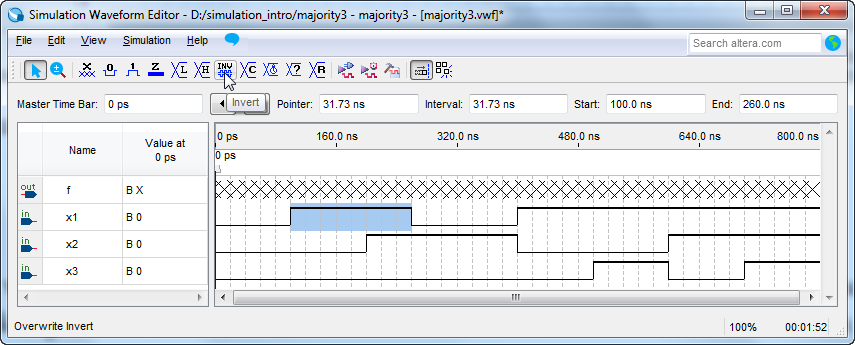
\includegraphics[scale=0.65]{figures/appendix/figure9.png}
	   \caption{Inverting the {\it x1} signal from 100 to 260 ns.} 
		 \label{fig:fig9}
		 \end{center}
	\end{figure}

	\item {\sf Count Value} \hbox{
\includegraphics[scale=0.7]{figures/appendix/icon10.png}}\\
	This tool allows a waveform to be partitioned into sections, in which the value is incremented 
	by a specified amount. 
	The {\sf Count Value} tool can only be applied to a single waveform or a grouped waveform (see section \ref{sec:grouping_and_ungrouping}).
	The options that are available when using the {\sf Count Tool} are illustrated in Figure~\ref{fig:fig10}. 
	\begin{figure}[H]
	   \begin{center}
	      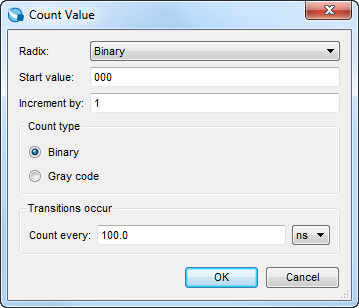
\includegraphics[scale=0.65]{figures/appendix/figure10.png}
	   \caption{Options available for for the {\sf Count Value} tool.} 
		 \label{fig:fig10}
		 \end{center}
	\end{figure}
	
	As an example, Figure~\ref{fig:fig11} shows the 3-bit input signal called {\it count} set to increment by one 
	every 100 ns. 
	\begin{figure}[H]
	   \begin{center}
	      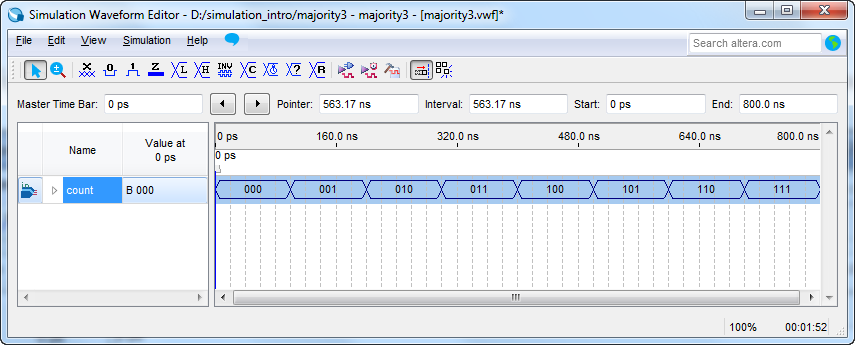
\includegraphics[scale=0.65]{figures/appendix/figure11.png}
	   \caption{An example of using the {\sf Count Value} tool.} 
		 \label{fig:fig11}
		 \end{center}
	\end{figure}
	
	\item {\sf Overwrite Clock} \hbox{
\includegraphics[scale=0.7]{figures/appendix/icon11.png}}\\
	This tool is used to generate a periodic waveform, which is often used as a clock signal. 
	The options available when using the {\sf Overwrite Clock} tool are shown in Figure~\ref{fig:fig12}. 
	\begin{figure}[H]
	   \begin{center}
	      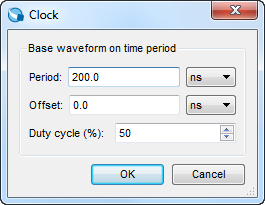
\includegraphics[scale=0.65]{figures/appendix/figure12.png}
	   \caption{Options available for the {\sf Overwrite Clock} tool.} 
		 \label{fig:fig12}
		 \end{center}
	\end{figure}
	
	In the example of Figure~\ref{fig:fig13}, the $x_3$ signal has been generated with a period of 200 ns, 
	an offset of 0 ns, and a duty cycle of 50\%. 
	\begin{figure}[H]
	   \begin{center}
	      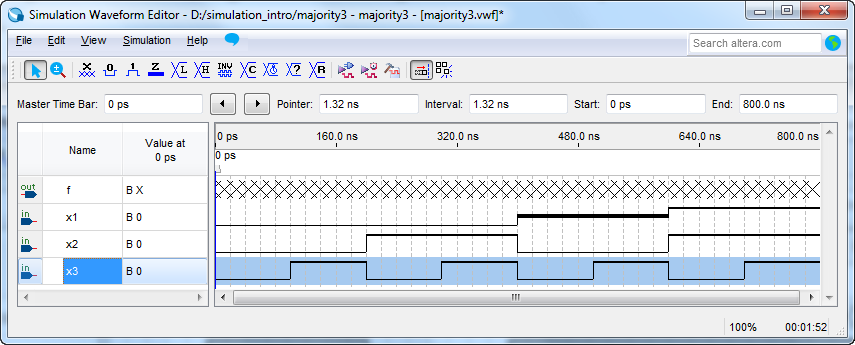
\includegraphics[scale=0.65]{figures/appendix/figure13.png}
	   \caption{An example of using the {\sf Overwrite Clock} tool.} 
		 \label{fig:fig13}
		 \end{center}
	\end{figure}

	\item {\sf Arbitrary Value} \hbox{
\includegraphics[scale=0.7]{figures/appendix/icon12.png}}\\
	This tool allows a signal to be set to an arbitrary value, which is particularly useful 
	for specifying the value of a multibit waveform. The options available when using 
	the {\sf Arbitrary Value} tool are shown in Figure~\ref{fig:fig14}. 
	\begin{figure}[H]
	   \begin{center}
	      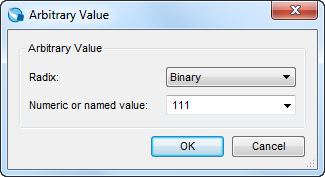
\includegraphics[scale=0.65]{figures/appendix/figure14.png}
	   \caption{Options available for for the {\sf Arbitrary Value} tool.} 
		 \label{fig:fig14}
		 \end{center}
	\end{figure}
	
	As an example, in Figure~\ref{fig:fig15} the {\it count} signal is set to three different 
	arbitrary binary values as specified by the user. 
	\begin{figure}[H]
	   \begin{center}
	      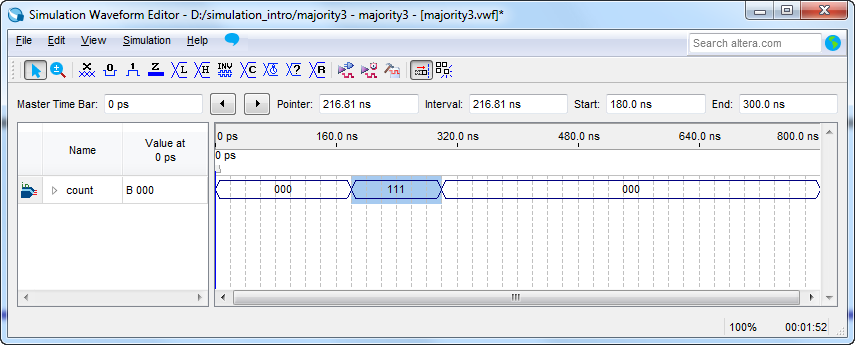
\includegraphics[scale=0.65]{figures/appendix/figure15.png}
	   \caption{The {\sf Arbitrary Value} tool is used to set values for the {\it count} signal.} 
		 \label{fig:fig15}
		 \end{center}
	\end{figure}
	
	\item {\sf Random Values} \hbox{\includegraphics[scale=0.7]{figures/appendix/icon13.png}}\\
	This tool assigns random values to the selected waveform(s), with several options as 
	shown in Figure~\ref{fig:fig16}.
	\begin{figure}[H]
	   \begin{center}
	      \includegraphics[scale=0.65]{figures/appendix/figure16.png}
	   \caption{Various options available for the Random Value tool.} 
		 \label{fig:fig16}
		 \end{center}
	\end{figure}
	
	For example, in Figure~\ref{fig:fig17}, the signal $x_1$ has been given random values.
	\begin{figure}[H]
	   \begin{center}
	      \includegraphics[scale=0.65]{figures/appendix/figure17.png}
	   \caption{An example of the {\sf Random Value} tool being used.} 
		 \label{fig:fig17}
		 \end{center}
	\end{figure}

	\item {\sf Snap to Grid} \hbox{\includegraphics[scale=0.7]{figures/appendix/icon14.png}}\\
	This option allows selections made with the {\sf Selection Tool} to snap to the light grey 
	grid lines running vertically down the waveform display. 
	This option can be toggled on and off by pressing the {\sf Snap to Grid button}. 
	It is set to on by default. Figure~\ref{fig:fig18} shows an example of the Selection Tool being 
	used with the Snap to Grid option turned off.
	\begin{figure}[H]
	   \begin{center}
	      \includegraphics[scale=0.65]{figures/appendix/figure18.png}
	   \caption{An example of the {\sf Snap to Grid} option turned off.} 
		 \label{fig:fig18}
		 \end{center}
	\end{figure}

	\item {\sf Snap to Transition} \hbox{\includegraphics[scale=0.7]{figures/appendix/icon15.png}}\\
	This option allows the {\sf Selection Tool} to automatically extend both the left and right sides of the selection rectangle outwards to the first transition encountered by any waveform in the editor. For example, with the {\sf Snap to Transition} option turned on, the {\sf Selection Tool} rectangle
	shown in Figure \ref{fig:fig19} would be expanded to create the selections illustrated in Figure \ref{fig:fig20}.
	This option can be toggled on and off by pressing the {\sf Snap to Transition} button, and is set to off 
	by default.
	\begin{figure}[H]
	   \begin{center}
	      \includegraphics[scale=0.65]{figures/appendix/figure19.png}
	   \caption{Making a selection with the {\sf Snap to Transition} option enabled.} 
		 \label{fig:fig19}
		 \end{center}
	\end{figure}
	\begin{figure}[H]
	   \begin{center}
	      \includegraphics[scale=0.65]{figures/appendix/figure20.png}
	   \caption{The expanded selection resulting from Figure \ref{fig:fig19}.} 
		 \label{fig:fig20}
		 \end{center}
	\end{figure}
	
\end{description}

\section{Using Multibit Signals}
This section describes features of the Simulation Waveform Editor that are useful for 
dealing with multibit signals.

\subsection{Grouping and Ungrouping Signals}
\label{sec:grouping_and_ungrouping}
Individual signals can be grouped together to create a multibit waveform. 
This is done by first selecting the desired waveforms by clicking on their names 
in the left side of the Waveform Editor with the key {\sf Ctrl} pressed as indicated in Figure~\ref{fig:fig21}.
Then, as shown in the figure, the grouping of signals is done by right-clicking on 
the selection and choosing {\sf Grouping $>$ Group...}.
\begin{figure}[H]
   \begin{center}
      \includegraphics[scale=0.65]{figures/appendix/figure21.png}
   \caption{An example of grouping signals.} 
	 \label{fig:fig21}
	 \end{center}
\end{figure}
In the options dialogue that opens, illustrated in Figure~\ref{fig:fig22}, a name must be 
assigned to the group, as well as a radix. In the example shown, the name {\it count} has been 
chosen with a binary radix.
\begin{figure}[H]
   \begin{center}
      \includegraphics[scale=0.65]{figures/appendix/figure22.png}
   \caption{Select a name and radix for the group of signals.} 
	 \label{fig:fig22}
	 \end{center}
\end{figure}

The resulting group of signals is shown in Figure~\ref{fig:fig23}. The multibit waveform can be expanded 
in the waveform editor to display its individual signals. 
\begin{figure}[H]
   \begin{center}
      \includegraphics[scale=0.65]{figures/appendix/figure23.png}
   \caption{An example of expanding a multibit signal.} 
	 \label{fig:fig23}
	 \end{center}
\end{figure}
A multibit signal can be ungrouped by right-clicking on the group of signals and selecting {\sf Grouping $>$ Ungroup...}.

It is also possible to create hierarchical groupings of signals as illustrated in Figure~\ref{fig:fig24}. In this example, 
the two bit signal called {\it level2} is combined with the signal called $x_3$ to create the three bit signal called {\it level1}.
It is only possible to group and ungroup top-level signals.
\begin{figure}[H]
   \begin{center}
      \includegraphics[scale=0.65]{figures/appendix/figure24.png}
   \caption{An example of hierarchical groups.} 
	 \label{fig:fig24}
	 \end{center}
\end{figure}

It is also possible to group input and output signals, as shown in Figure~\ref{fig:fig25}.
\begin{figure}[H]
   \begin{center}
      \includegraphics[scale=0.65]{figures/appendix/figure25.png}
   \caption{An example of grouping input and output signals.} 
	 \label{fig:fig25}
	 \end{center}
\end{figure} 

\subsection{Reverse Group or Bus Bit Order}
In Figure~\ref{fig:fig23}, the three bit signal count is displayed as the 3-tuple $x_1 x_2 x_3$. 
It is possible to reverse the order in which the bits are displayed as illustrated in Figure~\ref{fig:fig26}.
This is done by right-clicking on the name of the multibit signal and selecting {\sf Reverse Group or Bus Bit Order}, 
as seen in the figure.
\begin{figure}[H]
   \begin{center}
      \includegraphics[scale=0.65]{figures/appendix/figure26.png}
   \caption{Reversing the bit order on a group of signals.} 
	 \label{fig:fig26}
	 \end{center}
\end{figure} 

The effects of the bit reversal can be seen in Figure~\ref{fig:fig27}. The count waveform is now 
displayed as the 3-tuple $x_3 x_2 x_1$.
\begin{figure}[H]
   \begin{center}
      \includegraphics[scale=0.65]{figures/appendix/figure27.png}
   \caption{The result of reversing the bit order in Figure \ref{fig:fig26}.} 
	 \label{fig:fig27}
	 \end{center}
\end{figure} 	

\iffalse

\section{Displaying the Values of Finite State Machine (FSM) State Variables}
If a circuit includes a Finite State Machine (FSM), then it is possible to display the 
values of the corresponding state variables in the Simulation Waveform Editor. 
As an example, consider the fragment of Verilog code shown in Figure~\ref{fig:fig28}.
This code includes the definition of an FSM whose state variables are represented by the 
two-bit signal named {\it Tstep\_Q}. 

\begin{figure}[H]
\begin{center}
\begin{minipage}[t]{12.5 cm}
\begin{tabbing}
ZZ\=ZZ\=ZZ\=ZZ\=ZZ\=ZZ\=ZZ\=ZZ\=ZZ\kill
{\bf module} ~proc (DIN, Resetn, Clock, Run, Done, BusWires);\\
\>{\bf input} [15:0] DIN;\\
\>{\bf input} Resetn, Clock, Run;\\
\>{\bf output} Done;\\
\>{\bf output} [15:0] BusWires;\\
\>{\bf reg} [2:1] Tstep\_Q;\\
~\rule{5.0in}{0in}\\
\>{\bf parameter} T0 = 2'b00, T1 = 2'b01, T2 = 2'b10, T3 = 2'b11;\\
\>$\ldots$\\
~\\
\>// Control FSM state table\\
\>{\bf always} @(Tstep\_Q, Run, Done)\\
\>{\bf begin}\\
\>\>{\bf case} (Tstep\_Q)\\
\>\>\>T0: // data is loaded into IR in this time step\\
\>\>\>\>{\bf if} (!Run) Tstep\_D = T0;\\
\>\>\>\>{\bf else} Tstep\_D = T1;\\
\>\>\>T1: $\ldots$\\
\>\>{\bf endcase}\\
\>{\bf end}\\

\>$\ldots$\\

~\rule{5.0in}{0in}\\
\end{tabbing}
\end{minipage}
\end{center}
\caption{Fragment of example Verilog code.} 
\label{fig:fig28}
\end{figure}

This Verilog code can be included in a Quartus Prime project, 
which can then be compiled and simulated. The values of the {\it Tstep\_Q} signal can then 
be displayed in the Waveform Editor along with other signals in the circuit. However, a special 
process has to be used to insert the {\it Tstep\_Q} signal into the waveform display. Recall 
from Figures \ref{fig:fig6} and \ref{fig:fig7} that the {\sf Node Finder} tool is normally used 
as a convenient mechanism for importing signal names into the Waveform Editor. But for FSM 
state variables, it is not possible to use the {\sf Node Finder} tool. Instead, it is necessary 
to use the dialogue from Figure~\ref{fig:fig6} directly as illustrated in Figure~\ref{fig:fig29}.
Here, the name {\it Tstep\_Q} is manually typed into the name field, and
the type of signal is set by using the drop-down dialogue to {\sf MACHINE}. Clicking {\sf OK} 
in Figure~\ref{fig:fig29} imports the FSM signal into the Waveform Editor.
\begin{figure}[H]
   \begin{center}
      \includegraphics[scale=0.65]{figures/appendix/figure29.png}
   \caption{Specifying the {\it Tstep\_Q} signal in the {\sf Insert Node or Bus} window.} 
	 \label{fig:fig29}
	 \end{center}
\end{figure} 	

An example of simulation output that includes the {\it Tstep\_Q} signal is given in Figure~\ref{fig:fig30}.
This figure also shows the values of other signals in the circuit, which are needed in the simulation. 
Note that the values of Tstep\_Q are displayed in a symbolic manner, according to the state names which were 
given in the Verilog code in Figure~\ref{fig:fig28}.
\begin{figure}[H]
   \begin{center}
      \includegraphics[scale=0.65]{figures/appendix/figure30.png}
   \caption{Simulation results of the {\it Tstep\_Q} signal.} 
	 \label{fig:fig30}
	 \end{center}
\end{figure} 	

\fi


% Copyright and Trademark

%\newcommand{\datePublished}{Mar 2022}

\newcommand{\versnum}{21.1} %version number quartus/AMP
\newcommand{\quartusname}{Quartus\textsuperscript{\textregistered} Prime}	
\newcommand{\textBar}{For \quartusname{} \versnum{}}
\newcommand{\thisyear}{2022 } %for copyright
\newcommand{\company}{FPGAcademy.org}
\newcommand{\longteamname}{FPGAcademy.org}
\newcommand{\teamname}{FPGAcademy}
\newcommand{\website}{FPGAcademy.org}

\newcommand{\productAcronym}{AMP}
\newcommand{\productNameShort}{Monitor Program}

\newcommand{\productNameMedTM}{Monitor Program}
\newcommand{\productNameMed}{Monitor Program}

%\newcommand{\headerLogoFilePath}[1]{#1/FPGAcademy.png}



%%%%%%%%%%%%%%%%%%%%%%%%%%%%%%%%%%%%%%%%
%%% FPGAcademy Copyright Information %%%
%%%%%%%%%%%%%%%%%%%%%%%%%%%%%%%%%%%%%%%%

%Always put the copyright on a new page (clear page), with some vertical space from top
\clearpage
\vspace{1in}

\noindent

Copyright {\copyright} FPGAcademy.org. All rights reserved. FPGAcademy and the FPGAcademy logo are trademarks of  FPGAcademy.org.  This document is being provided on an ``as-is'' basis and as an accommodation and therefore all warranties, representations or guarantees of any kind (whether express, implied or statutory) including, without limitation, warranties of merchantability, non-infringement, or fitness for a particular purpose, are specifically disclaimed.

%FPGAcademy assumes no responsibility or liability arising out of the application or use of any information,  product,  or  service  described  herein  except  as  expressly  agreed  to  in  writing  by  FPGAcademy.



**Other names and brands may be claimed as the property of others.




\end{document}
